\documentclass[]{article}
\usepackage{graphicx}
\graphicspath{{./images/}}
%opening
\title{Google Maps \& GPS}
\author{Junchao Zhou \and Matthew Swartwout \and James Zhang }

\begin{document}

\maketitle

\section{Homework 1}
Homework 1 requires us to make “TAKE A PICTURE” button functional. After clicking this button, a camera activity should be opened which allows us to take a photo and save it to a specific directory under external storage. 
In order to open another activity in the current activity, we need to use Intent class to tell our current activity what operation we want to perform. In the function below

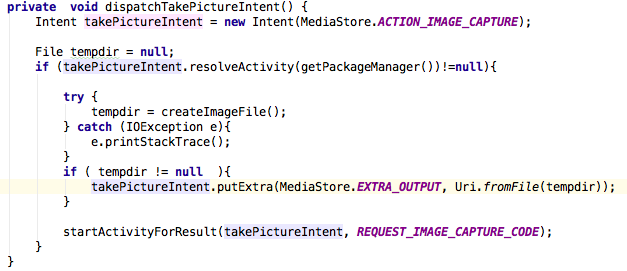
\includegraphics[keepaspectratio, width=\textwidth]{codeSnippet1}

MediaStore.ACTION\_IMAGE\_CAPTURE is a standard intent action, which can be used to have the camera application capture an image and return it. Then we need to specify a storage directory for saving the image. We use a function createImageFile() to return the storage path for the taken photo and use putExtra(MediaStore.EXTRA\_OUTPUT, Uri.fromFile(tempdir)) to save the image to the file path specified by the Uri.

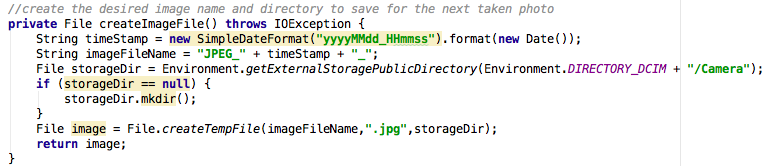
\includegraphics[keepaspectratio, width=\textwidth]{codeSnippet2}

However, to get the thumbnails and display them on the map, we can’t use putExtra() because once the image is saved by using putExtra(),  then in onActivityResult(…) function data.getExtras() will return null. So we need other approach to save the thumbnail.
  
\section{Homework 2}
For Homework 2, we used the application to take photos of ten different buildings around campus. For each photo, the application saves the timestamp and the GPS coordinates(latitude and longitude) into a CSV file in the DCIM folder. The Android Camera encodes each photo in data of type Intent. This data is used by the onActivityResult method. If the photo was successfully captured, the method saves the timestamp and the last available coordinate data to the CSV file. The method then sets the photo data as an imageBitmap, which is compressed in to a .PNG file. Lastly, the method adds a marker to the Google Map mMap with the coordinates for the marker position and the photo as the icon.
\section{Homework 3}
For getting the thumbnails, we implemented two separate methods. The first creates a marker and gets the thumbnail for a photo immediately after it is taken. The second checks to see if any thumbnails exist when the app is first launched (i.e. photos were taken with the app on a previous execution) and creates those markers.

For the first example, creating a marker immediately after the photo is taken, we added code to onActivityResult. After the CSV file is written to, we added the example code given to getExtras and extract the Bitmap. Then the file is named JPEG\_TIMESTAMP\_.jpg and stored in the DCIM/Camera directory. Finally, a marker is added to the map with the thumbnail at the latitude and longitude coordinates.

For the second example, creating markers that were previously taken, we added code to setUpMap. First we set up a BufferedReader from our Homework2.csv file. Then, we loop through each line of the file, knowing that each line consists of TIMESTAMP, LATITUDE, LONGITUDE. We read the TIMESTAMP and create a filepath based off that. Then we add a marker with that thumbnail, at the corresponding Latitude and Longitude for that Timestamp. 
\section{Homework 4}
\section{Screenshots}
\section{Division of Work}
\end{document}
